\documentclass[oneside, 11pt]{article}

\usepackage[T1]{fontenc}
\usepackage[utf8]{inputenc}
\usepackage[english]{babel}

\usepackage{fouriernc}
\usepackage[detect-all, binary-units, separate-uncertainty=true,
            per-mode=symbol, retain-explicit-plus, retain-unity-mantissa=false]{siunitx}

\usepackage{setspace}
\setstretch{1.2}

\setlength{\parskip}{\smallskipamount}
\setlength{\parindent}{0pt}

\usepackage[headheight=14pt]{geometry}
\geometry{marginparwidth=0.5cm, verbose, a4paper, tmargin=3cm, bmargin=3cm,
          lmargin=2cm, rmargin=2cm}

\usepackage{float}

\usepackage[fleqn]{amsmath}
\numberwithin{equation}{section}
\numberwithin{figure}{section}

\usepackage{graphicx}
\graphicspath{{images/}{../../../images/}}

\usepackage{tikz}
\usetikzlibrary{shapes}
\usetikzlibrary{plotmarks}

\newcounter{Exercise}
\setcounter{Exercise}{1}
\usepackage{xcolor}
\definecolor{shadecolor}{gray}{0.9}
\usepackage{framed}
\usepackage{caption}

\usepackage{url}


\usepackage{fancyhdr}
\pagestyle{fancy}
\fancyhf{}
\rhead{\thepage}
\renewcommand{\footrulewidth}{0pt}
\renewcommand{\headrulewidth}{0pt}

\fancypagestyle{firststyle}
{
    \fancyhf{}
    \rhead{\thepage}
    \cfoot{
\includegraphics[height=30pt]{HiSPARClogo}}
    \rfoot{
\includegraphics[height=25pt]{CCbysa}}
    \lfoot{
\includegraphics[height=30pt]{NIKHEFlogo}}
    \renewcommand{\footskip}{50pt}
    \renewcommand{\footrulewidth}{0.1pt}
    \renewcommand{\headrulewidth}{0pt}
}

\newcommand{\figref}[1]{Figuur~\ref{#1}}

\newcommand{\hisparc}{\textsmaller{HiSPARC}\xspace}
\newcommand{\kascade}{\textsmaller{KASCADE}\xspace}
\newcommand{\sapphire}{\textsmaller{SAPPHiRE}\xspace}
\newcommand{\jsparc}{\textsmaller{jSparc}\xspace}
\newcommand{\hdf}{\textsmaller{HDF5}\xspace}
\newcommand{\aires}{\textsmaller{AIRES}\xspace}
\newcommand{\csv}{\textsmaller{CSV}\xspace}
\newcommand{\python}{\textsmaller{PYTHON}\xspace}
\newcommand{\corsika}{\textsmaller{CORSIKA}\xspace}
\newcommand{\labview}{\textsmaller{LabVIEW}\xspace}
\newcommand{\daq}{\textsmaller{DAQ}\xspace}
\newcommand{\adc}{\textsmaller{ADC}\xspace}
\newcommand{\hi}{\textsc{h i}\xspace}
\newcommand{\hii}{\textsc{h ii}\xspace}
\newcommand{\mip}{\textsmaller{MIP}\xspace}
\newcommand{\hisparcii}{\textsmaller{HiSPARC II}\xspace}
\newcommand{\hisparciii}{\textsmaller{HiSPARC III}\xspace}

\DeclareSIUnit{\electronvolt}{\ensuremath{\mathrm{e\!\!\:V}}}

\DeclareSIUnit{\unitsigma}{\ensuremath{\sigma}}
\DeclareSIUnit{\mip}{\textsmaller{MIP}}
\DeclareSIUnit{\adc}{\textsmaller{ADC}}

\DeclareSIUnit{\gauss}{G}
\DeclareSIUnit{\parsec}{pc}
\DeclareSIUnit{\year}{yr}



\begin{document}

\title{Fluorescentie}
\author{dr. Th. W. Kool, N.G. Schultheiss}
\date{}

\maketitle
\thispagestyle{firststyle}

\section{Inleiding}

Deze module volgt op de module ``de Broglie''. Het detecteren van
kosmische straling in onze ski-boxen geschiedt met behulp van het
organische molecuul antraceen met molecuulformule: $\mathrm{C}_{14}\mathrm{H}_{10}$.

\begin{figure}[h]
\noindent \begin{centering}
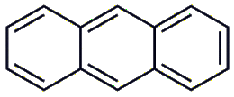
\includegraphics[scale=0.8]{Anthraceen-schematisch}
\par\end{centering}

\caption{\label{fig:Structuurformule-Anthraceen}De structuurformule van Anthraceen}
\end{figure}


Op de hoekpunten van de ring bevinden zich de C atomen. Elk streepje
in \figref{fig:Structuurformule-Anthraceen} stelt 2 elektronen
voor. Bovenstaand plaatje is eigenlijk niet correct, omdat bij de
dubbele bindingen de elektronen vast zitten, hetgeen in de praktijk
niet het geval is. Tussen de atomen bevinden zich 2 elektronen, maar
daar C een covalentie van 4 heeft ontbreken er nog in totaal 14 elektronen.
Die kunnen zich vrij bewegen over de 3 ringen. Dit is te zien in
\figref{fig:Anthraceen2}.

\begin{figure}[h]
\noindent \begin{centering}
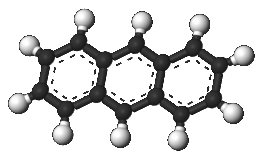
\includegraphics[scale=0.8]{Anthraceen}
\par\end{centering}

\caption{\label{fig:Anthraceen2}Een betere voorstelling van Anthraceen}
\end{figure}


\section{Atoombouw}

Om te begrijpen hoe \emph{fluorescentie} tot stand komt zullen we
eerst iets over de \emph{bouw van atomen} en de opbouw van het periodiek
systeem moeten weten. Daarna kunnen we de \emph{chemische binding}
beschouwen.

Rutherford beschreef een atoom als een positieve kern met daar omheen
cirkelende elektronen.


\paragraph*{Opdracht 1:}

\emph{Uit welk experiment haalde Rutherford zijn ideeën?}

Volgens het model van Bohr bewegen de elektronen in banen (orbits)
om de kern, net zoals de bewegingen van de planeten om de zon. Volgens
berekeningen met behulp van de wetten uit de klassieke mechanica (Newton)
kwam hij erop dat de elektronen zich in verschillend banen bewogen,
n.l. de K-, L-, M-schil enz. De opvulling geschiedt volgens de volgende
formule: $2\mathrm{n}^{2}$, met n een geheel getal. Zo kan de K-schil
2, de M-schil 8 en de N-schil 18 elektronen bevatten. In het periodiek
systeem heet dat periode. Veel eigenschappen van de atomen kunnen
hierdoor begrepen worden.

\begin{figure}[h]
\noindent \begin{centering}
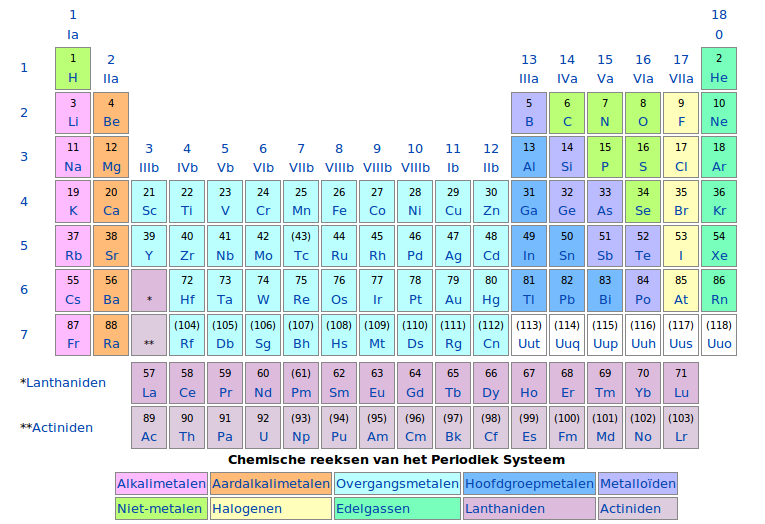
\includegraphics[width=14cm]{Mendeljev}
\par\end{centering}

\caption{Het periodiek systeem}
\end{figure}


Nadat de Broglie het idee gepostuleerd had dat deeltjes golfkarakter
hadden en golven deeltjes karakter bezaten, hetgeen later in experimenten
bevestigd werd, ontstond langzamerhand de moderne kwantummechanica.


\paragraph*{Opdracht 2:}

\emph{Geef een synoniem voor postuleren.}

Met behulp van de beroemde Schrödinger golfvergelijking was men in
staat om van het H-atoom exact de banen van de elektronen en de bijbehorende
energie niveaus te berekenen. Dit was een enorme doorbraak in de natuurkunde.

De golfvergelijking luidt:

\begin{equation}
H\psi=E\psi
\end{equation}


Dit is een z.g.n. $2^{\mathrm{de}}$ orde differentiaalvergelijking.
De hamiltoniaan \emph{H} bevat termen voor de beweging van de kernen
en de elektronen, alsmede de interacties tussen de kernen onderling,
de elektronen onderling en de kernen met elektronen. De energieën
\emph{E} kunnen ook gevonden worden. $\psi$ is de zogenaamde golffunctie.
We zullen hierop terugkomen.


\paragraph*{Opdracht 3:}

\emph{Welke interacties (krachten) zullen de kernen en elektronen
hebben?}


\paragraph*{Opdracht 4:}

\emph{Welke formule in de mechanica van Newton geeft de energie voor
beweging?}

De oplossingen van deze $2^{\mathrm{de}}$ orde differentiaal vergelijking
zijn niet eenvoudig te vinden, maar o.a. de banen van de elektronen
met bijbehorende gekwantiseerde energieën kunnen berekend worden.
De banen, waarin de elektronen zich bevinden zijn:

\begin{equation}
\begin{array}{c}
1s\\
2s,2p_{x},2p_{y},2p_{z}\\
3s,3p_{x},3p_{y},3p_{z},3d\\
enz.
\end{array}
\end{equation}


\emph{}
\begin{figure}[h]
\noindent \begin{centering}
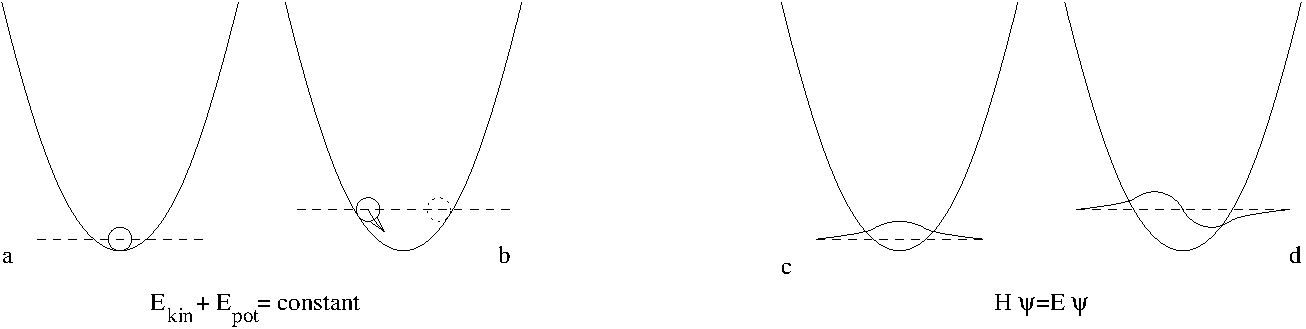
\includegraphics[scale=0.7]{energieGolf}
\par\end{centering}

\emph{\caption{\label{fig:Energie-en-golfvergelijking}Energie en golfvergelijking}
}
\end{figure}


In igref{fig:Energie-en-golfvergelijking} zijn de energie en
golfvergelijking voor de grondtoestand (a \& c) en de eerste aangeslagen
toestand (b \& d) van een harmonische oscillator te zien. Voorbeelden
van harmonische oscillatoren zijn bijvoorbeeld een slinger, een massa-veer
systeem of een kogel op een parabolische baan. Als we de situatie
in \figref{fig:Energie-en-golfvergelijking}b bekijken zien we dat de
potentiele energie bij de maximale uitwijking ook maximaal is. Deze
wordt omgezet in kinetische energie, die maximaal is in het midden.


\paragraph*{Opdracht 5:}

\emph{We kijken op een willekeurig moment naar }\figref{fig:Energie-en-golfvergelijking}b\emph{,
leg uit waar je het deeltje waarschijnlijk waarneemt.}

De diagrammen in \figref{fig:Energie-en-golfvergelijking}c en \figref{fig:Energie-en-golfvergelijking}d
geven de oplossing van de $2^{e}$ orde differentiaalvergelijking
$H\psi=E\psi$. Ook hier kan de kans worden gevonden om een deeltje
waar te nemen. Deze kans is te berekenen met $\psi^{2}$.


\section{Spin}

Nu was al eerder in experimenten met H atomen en inhomogene magneetvelden
aangetoond dat een elektron slechts twee standen in de ruimte kan
innemen. Dit werd de elektronen spin S genoemd (to spin = draaien).
Hierbij gaat een magneetveldje gepaard (zie igref{fig:Spin}).


\paragraph*{Opdracht 5:}

\emph{Leg uit wat N en S in igref{fig:Spin} betekenen. Teken
de veldlijnen.}

\begin{figure}[h]
\noindent \begin{centering}
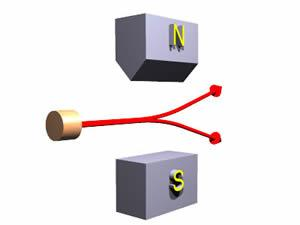
\includegraphics[width=5.5cm]{spin}
\par\end{centering}

\caption{\label{fig:Spin}Spin}
\end{figure}


Om de opbouw van het periodiek systeem te begrijpen introduceerde
Pauli zijn regel dat alleen elektronen met tegengestelde spin in een
baan kunnen bevinden $S=\pm\frac{1}{2}(\frac{h}{2\pi})$. Hierbij
is h de constante van Planck. Deze waarde is te vinden in Binas.

Zo kan er in de eerste schil (nu orbitaal genaamd) zich maximaal 2
elektronen bevinden (He). In de tweede schil maximaal 8, maar wel
verdeeld over de $2s$, $2p_{x}$, $2p_{y}$ en $2p_{z}$ banen (zie
periodiek systeem).

Laten we het H-atoom eens nader bekijken: H heeft atoomnummer 1. Het
elektron bevindt zich als het in de laagste energie toestand zit in
de 1s orbitaal. In igref{fig:Orbitalen} zijn de orbitalen van
de verschillende banen getekend. De bijbehorende energieniveaus zijn
in igref{fig:Energieniveaux}.

\begin{figure}[h]
\noindent \begin{centering}
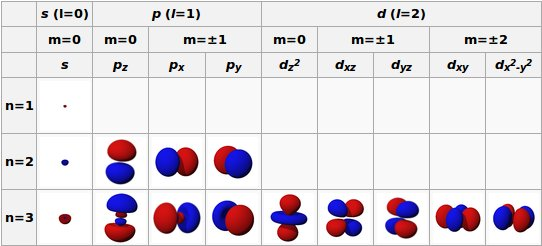
\includegraphics[width=10cm]{Orbitalen}
\par\end{centering}

\caption{\label{fig:Orbitalen}Orbitalen}
\end{figure}


\begin{figure}[h]
\noindent \begin{centering}
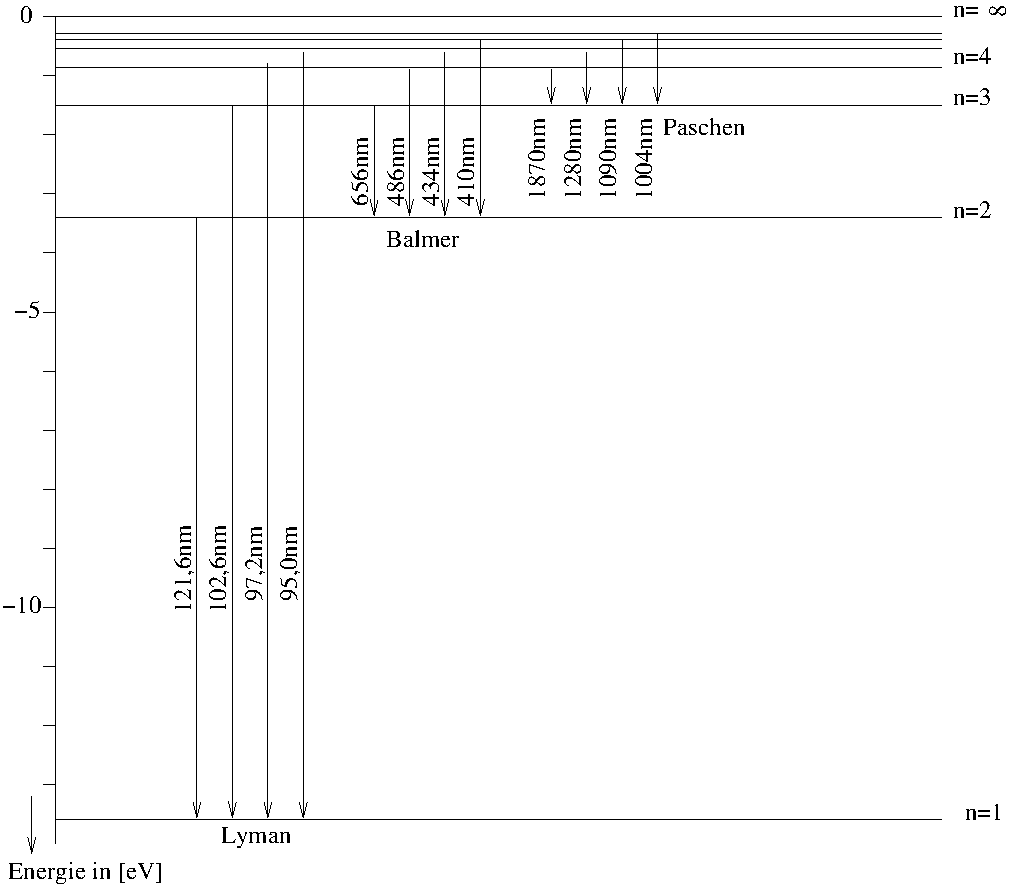
\includegraphics[scale=0.65]{waterstof}
\par\end{centering}

\caption{\label{fig:Energieniveaux}Vervalreeksen in waterstof}
\end{figure}


Energie in de vorm van straling kan door het atoom opgenomen worden.
Dit wordt absorptie genoemd en energie in de vorm van straling kan
worden afgestaan. Dit wordt emissie genoemd. De pijlen in igref{fig:Energieniveaux}
zijn de emissielijnen van het H-atoom. 


\section{Singulet versus triplet}

\begin{figure}[h]
\noindent \begin{centering}
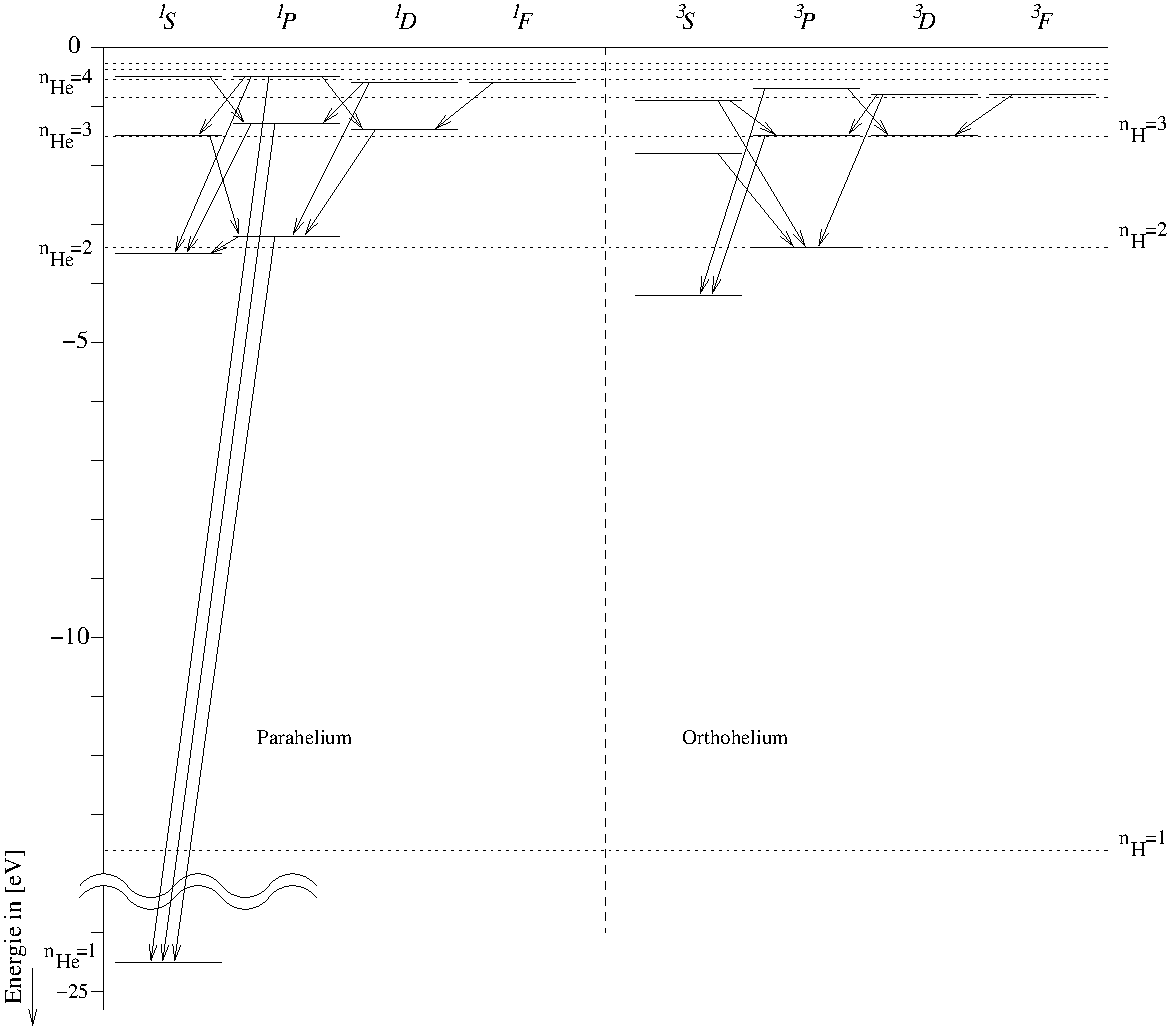
\includegraphics[scale=0.65]{helium}
\par\end{centering}

\caption{\label{fig:Singulet-en-triplet}Singulet en triplet verval}
\end{figure}


Laten we nu naar het He-atoom kijken. We hebben te maken met 2 elektronen.
Deze kunnen volgens Pauli zich in de grondtoestand (laagste energie)
bevinden met tegengestelde spin. Nu komen we tot een nieuw begrip
in de moderne natuurkunde, n.l. de elektronen zijn ononderscheidbaar.
Dus we weten niet waar welk elektron zich bevindt.

Wiskundig formuleren \footnote{De functie 1\emph{s}(1) wil zeggen dat
atoom 1 in de baan 1\emph{s} zit. De eerste term geeft de kans dat de
elektronen 1 en 2 in een bepaalde toestand zitten. Omdat we door de
onbepaaldheid niet weten of dit op deze manier gebeurd, trekken we hier
de kans af dat de spin verwisseld is.} we dit als volgt, waarbij
$\alpha$ spin-up (omhoog) en $\beta$ spin-down (omlaag) betekent:

\begin{equation}
N\{1s(1)\alpha(1)1s(2)\beta(2)-1s(1)\beta(1)1s(2)\alpha(2)\}
=N\{1s(1)1s(2)[\alpha(1)\beta(2)-\beta(1)\alpha(2)]\}
\end{equation}


Het eerste elektron heeft label 1 en het tweede elektron heeft label
2. Bovenstaande uitdrukking noemen we een \emph{golffunctie} $\psi$.


\paragraph*{Opdracht 6:}

\emph{Leg in eigen woorden uit wat} $1s(1)\alpha(1)1s(2)\beta(2)$
\emph{natuurkundig betekent.}

We zien in de formule dat elk elektron met $\alpha$-spin is gepaard
met een elektron met $\beta$-spin.


\paragraph*{Opdracht 7:}

\emph{Wat betekent dit voor het totale magnetische moment?}

Deze gepaarde toestand noemen we een \emph{singulet}.

We beschouwen nu He in de eerste aangeslagen toestand. De elektronen
kunnen zich nu in zowel de 1s als de 2s baan bevinden met hun respectievelijke
spins.

We zullen alleen naar het spindeel kijken en niet naar het baandeel
(anders wordt het voor nu te gecompliceerd). In formule \ref{eq:HeAangeslagen}
zien we de golffuncties van het aangeslagen He (alleen het spindeel):

\begin{equation}
\begin{array}{c}
N\{\alpha(1)\alpha(2)\}\\
N\{\beta(1)\beta(2)\}\\
N\{\alpha(1)\beta(2)+\beta(1)\alpha(2))\}\\
N\{\alpha(1)\beta(2)-\beta(1)\alpha(2))\}
\end{array}\label{eq:HeAangeslagen}
\end{equation}


\paragraph*{Opdracht 8:}

\emph{Wat denk je dat het totale spin moment van de vier uitdrukkingen
in formule \ref{eq:HeAangeslagen} is?}

De eerste drie formules vormen een zogenaamde \emph{triplet} (magnetisch)
en de laatste een \emph{singulet} (niet magnetisch).

In igref{fig:Singulet-en-triplet} is het energiediagram van
He weergegeven. Het linker gedeelte wordt door de singuletten gevormd.
Het rechter gedeelte door de tripletten.


\section{De binding in het waterstofmolecuul}

Hoe kunnen wij de chemische binding in de kwantumfysica voorstellen?
Allereerst bekijken we het molecuul $\mathrm{H}_{2}$. De \emph{1s}
van het ene atoom met de \emph{1s} van het andere atoom vormt een
moleculaire baan. Zowel de + als de \textendash{} combinatie is mogelijk.

De volgende combinaties zijn mogelijk tussen atoom \emph{a} en atoom
\emph{b}:

\begin{equation}
\varphi=N\{1s(a)\pm1s(b)\}
\end{equation}


Hierin is de + combinatie bindend (bonding) en de \textendash{} combinatie
anti-bindend (anti-bonding) en ligt ook hoger in energie.

Ieder H-atoom in $\mathrm{H}_{2}$ heeft een elektron tot zijn beschikking,
hierdoor bevinden zich in de bindende moleculaire baan twee elektronen
met tegengestelde spin (volgens het Pauli-principe). Zie figuuronderstaand
diagram.

\begin{figure}[h]
\noindent \begin{centering}
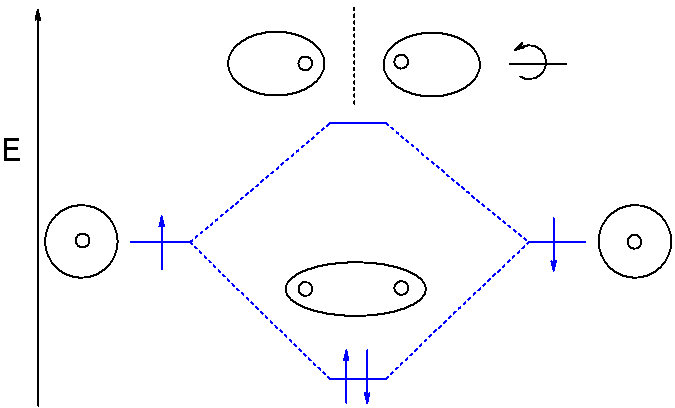
\includegraphics[width=4.5cm]{H2ST}
\par\end{centering}

\caption{Spin in een waterstof molecuul}
\end{figure}


In de aangeslagen toestand kunnen er weer triplet en singulet toestanden
voor komen.


\paragraph*{Opdracht 9:}

\emph{Teken in bovenstaand diagram de aangeslagen toestanden en schrijf
de bijbehorende spin-golffuncties op.}

Moleculen trillen ook en dat geeft aanleiding tot andere energieniveaus
(sneller en langzamer trillen).

\begin{figure}[h]
\noindent \begin{centering}
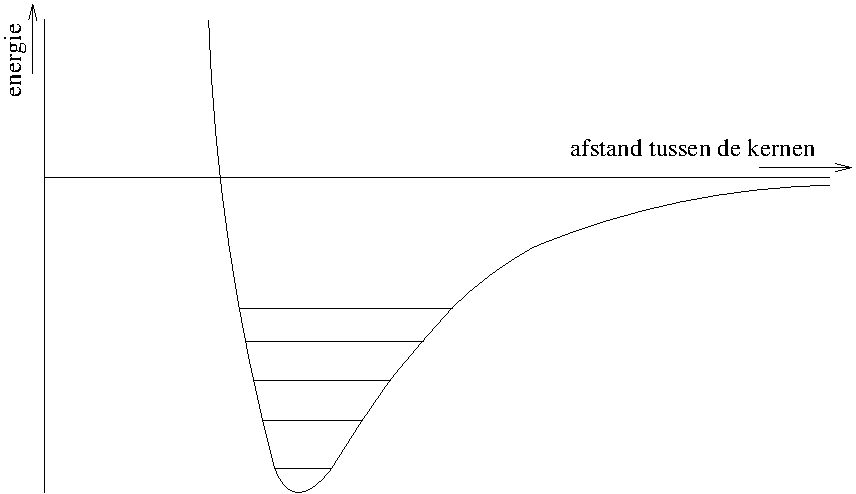
\includegraphics[scale=0.65]{molecuulenergie}
\par\end{centering}

\caption{De energieniveaus van een waterstofmolecuul}
\end{figure}


De horizontale as van de figuur geeft de afstand tussen de H-atomen
aan, de verticale as de energie. Er is dus een meest gunstige afstand
waarop de atomen van elkaar verwijderd zijn om te binden. De figuur
die op een parabool lijkt is stelt de verschillende energieën voor,
die het twee-atomige molecuul kan innemen. De energieniveaus, die
daarin getekend zijn, stellen de trillingsenergieën (vibraties) voor.


\section{Bindingen in anthraceen}

Nu stappen we over op het koolstofatoom dat deel uitmaakt van het
antraceenmolekuul. C heeft atoomnummer 6. In de 1s orbital bevindt
zich 2 elektronen en in de $2s$, $2p_{x}$ $2p_{y}$ $2p_{z}$ de
overige 4 elektronen. In elk van de orbitals bevindt zich nu 1 elektron.


\paragraph*{Opdracht 10:}

\emph{Heb je een idee waarom er zich maar 1 elektron in elk van de
2s en 2p banen bevindt, terwijl er volgens het Pauli principe er zich
maximaal 2 elektronen met tegengestelde spin in iedere baan kunnen
bevinden?}

\begin{figure}[h]
\noindent \begin{centering}
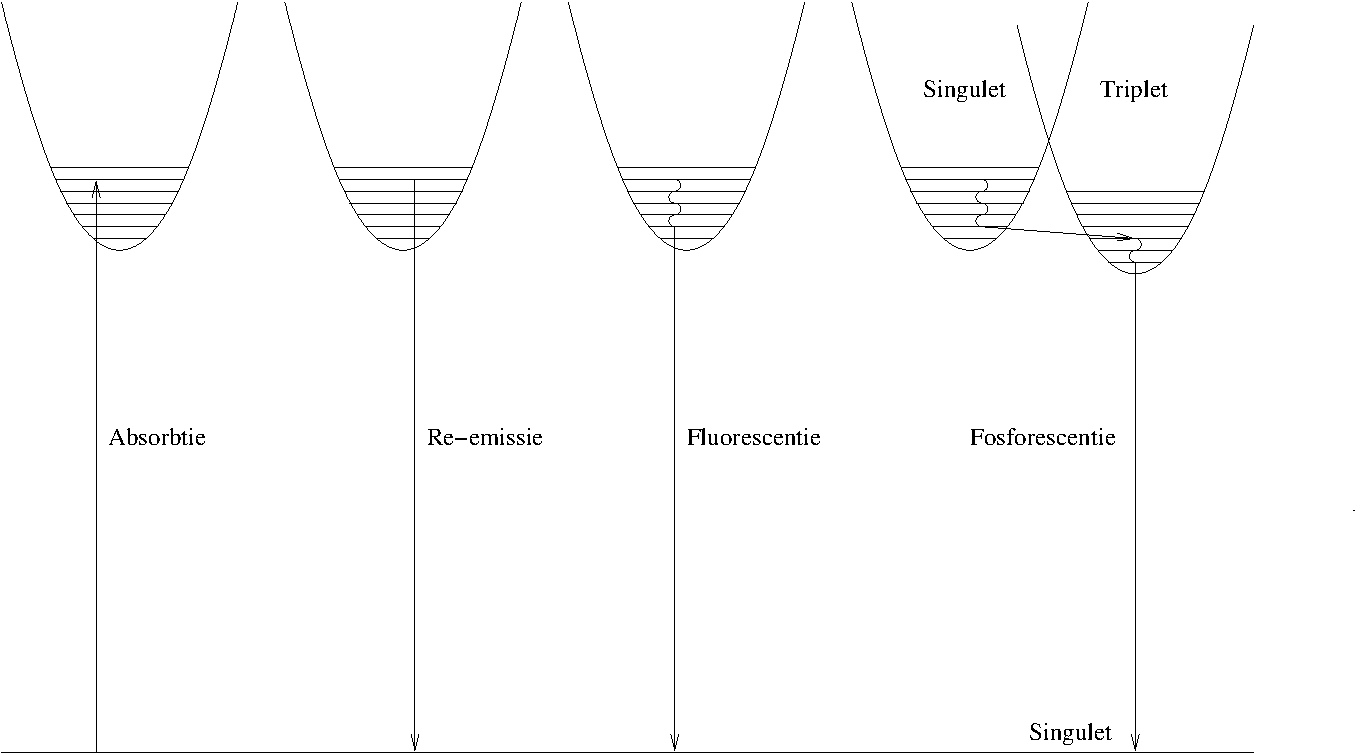
\includegraphics[scale=0.65]{hetoestanden}
\par\end{centering}

\caption{\label{fig:Verval-in-He}Verval in een molecuul}
\end{figure}


Als we nu naar het antraceen molecuul kijken hebben we bindingen tussen
de C atomen onderling en tussen de C en H atomen.

De laag in energie liggende 1s banen van het C-atoom beschouwen niet.
Deze dragen niet bij aan de chemische binding. We beschouwen alleen
de 1s van het H-atoom en de $2s$ en $2p_{x,y,z}$ banen van het C-atoom.

De C-H bindingen worden gevormd door de 1s van het H-atoom en de $p_{x}$
van het C-atoom. De C-C bindingen worden gevormd door de $p_{y}$
van de C-atomen. Deze liggen in het vlak van het molecuul. In de chemie
worden dit $\sigma$-bindingen genoemd. De $p_{z}$ vormen de zogenaamde
$\pi$\textendash{}bindingen. Deze staan loodrecht op het vlak van
het molecuul.


\paragraph*{Opdracht 11:}

\emph{Teken de $p_{z}$ banen in het antraceen molecuul.}

Fluorescentie en (fosforescentie) in antraceen heeft alleen te maken
met de $\pi$\textendash{}elektronen.We beschouwen nu de buitenste
twee $\pi$\textendash{}elektronen. De rest van de elektronen vormen
paren, volgens het Pauli-principe. Deze twee elektronen kunnen zich
weer hetzelfde verdelen als de elektronen in He, namelijk een singulet
grondtoestand, en aangeslagen singulet en triplet toestanden.

Fluorescentie is alleen mogelijk tussen een aangeslagen singulet toestand
en een singulet grondtoestand. Dit geschiedt in $10^{-8}$s. Fosforescentie
is eigenlijk \textquoteleft{}verboden\textquoteright{} en duurt daarom
\textquoteleft{}\textquoteright{}veel\textquoteright{}\textquoteright{}
langer. Deze vindt plaats tussen een triplet toestand en de singulet
grondtoestand. Als energie wordt geabsorbeerd valt het eerst via de
vibratie toestanden terug en valt dan middels het uitzenden van een
lichtfoton terug naar de grondtoestand.


\paragraph*{Opdracht 12:}

\emph{Leg igref{fig:Verval-in-He} uit.}

Het energiediagram in igref{fig:Verval-in-Anthraceen} geeft
de mogelijke energie overgangen in het antraceen molecuul weer.

\begin{figure}[h]
\noindent \begin{centering}
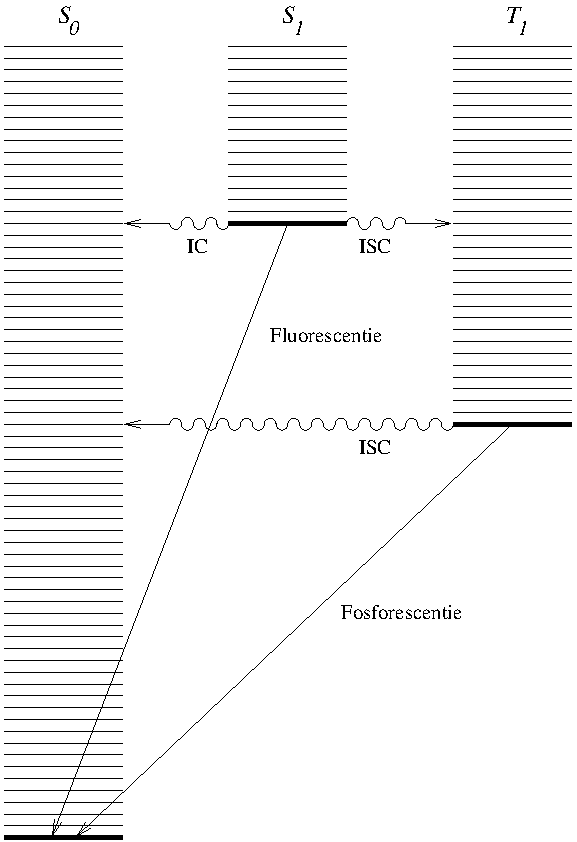
\includegraphics[scale=0.65]{anthraceentoestanden}
\par\end{centering}

\caption{\label{fig:Verval-in-Anthraceen}Verval in Anthraceen}
\end{figure}


ISC betekent intersystem crossing. Overgangen van de aangeslagen singulet
toestand naar de vibraties (trillingen van de triplettoestand. IC
betekent internal conversion. Overgang van de aangeslagen singulet
toestand naar de vibraties van de singulet grondtoestand.


\paragraph*{Opdracht 13:}

\emph{Wat valt je op met betrekking tot de vibratieniveaus van de
$S_{0}$ (singulet grondtoestand) en de $S_{1}$ (eerste aangeslagen
singulet toestand).}

Fluorescentie vindt plaats van de aangeslagen singulet toestand ($\pi^{*}$)
naar de singulet grondtoestand ($\pi$). Dit nemen we waar in het
antraceen molecuul.


\paragraph*{Opdracht 14:}

\emph{Waarom wordt hier het symbool $\pi^{*}$ gebruikt?}

\end{document}
